\section{IP address allocation dynamics}
\label{sec:allocations}

\subsection{Allocated IP block sizes}

The distribution of allocated block sizes has changed over the past six years,
as shown in figure \ref{fig:IP allocations}. The number of allocations has
increased for every prefix prefix length, but at different rates. In 2003, /24
was the most popular size, as it is today, but there were only about half as
many /20 allocations as /19 ones, whereas in 2008 they were about the same.
There has been almost no increase in /16 blocks. This shows the growing trend
towards smaller blocks as the IPv4 address space approaches saturation.
Throughout the six-year period, most IP allocations are /24 blocks. The next
most popular block size is /16, followed by /19 and /20. The smaller block
sizes (/19 and smaller) have had a larger increase in usage than /16, /17, and
/18.

\begin{figure}[htbp]
 	\centering
 		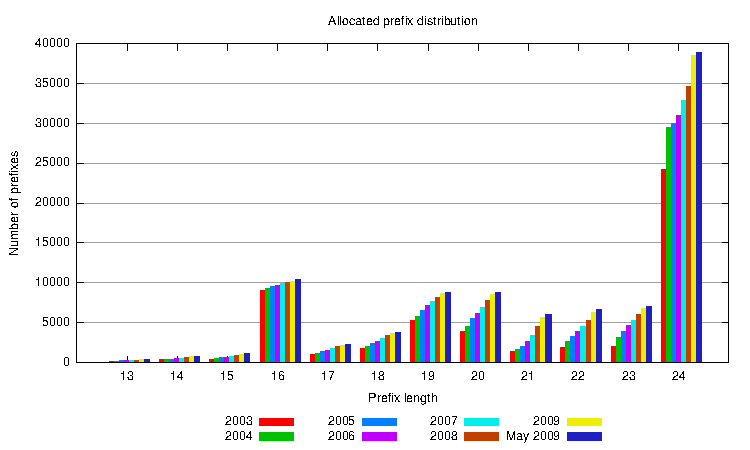
\includegraphics[width=0.5\textwidth]{02_prefixes/02_ip_prefixes_zoom}
	\caption{Allocated prefix distribution}
 	\label{fig:IP allocations}
\end{figure}

\subsection{Yearly distribution of IP allocations}

% \begin{figure}[htbp]
%  	\centering
%  		 \includegraphics[width=0.5\textwidth]{04_plus_minus/addremoveprefixallocculmulative}
% 	\caption{Trends in IP prefix allocation}
%  	\label{fig:IP allocations new and gone}
% \end{figure}

Figure \ref{fig:IP allocations new and gone} shows that the number of
allocated IP prefixes has increased by over 40,000 in the past six years. Some
of the increase was due to new allocations, while a smaller amount was due to
prefix splitting (where one prefix was split into smaller prefixes). Not all
changes increased the number of allocations, however. Some prefixes
disappeared in the same time period, although the number of new ones greatly
outpaced the disappearances. Another dynamic which did not directly affect the
number of allocations was prefix extension, where an existing prefix increased
its size by including adjacent, unallocated address space (e.g. a /16 prefix
might become a /15 prefix by including the adjacent /16 address space).

\begin{figure}[htbp]
    \centering
        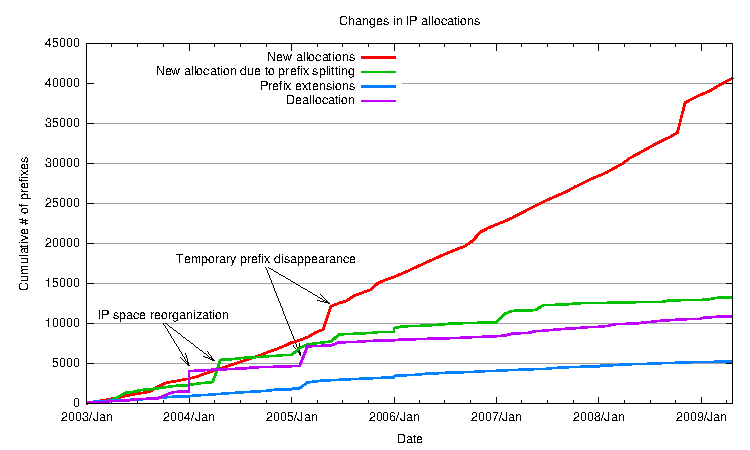
\includegraphics[width=\columnwidth]{04_3_plus_minus/changes}
    \caption{Changes in IP allocations}
    \label{fig:IP allocations new and gone}
\end{figure}

Figure \ref{fig:alloc ages total} plots the number of prefixes allocated each
year, according to snapshots taken in the years from 2003 to 2009 (shown in
different colors). It is interesting to note that the number of prefixes
allocated in the 90s has increased since then, especially in the past year.
This is the effect of prefix splitting, where a larger allocated block is
split into multiple blocks. When blocks are split, the resulting blocks retain
the year of origin as the block they were part of. The graph shows that many
of the existing allocations originated in the 90s, but also suggests that many
of these are split pieces of the fewer, larger blocks that were actually
allocated back then.

\begin{figure}[htbp]
	\centering
		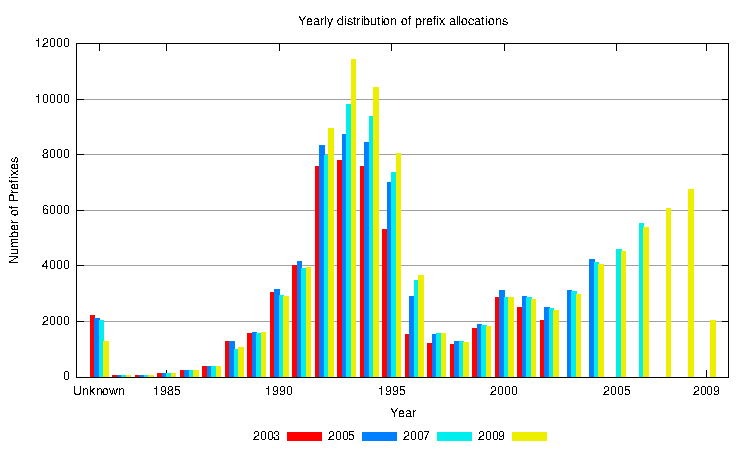
\includegraphics[width=\columnwidth]{10_alloc_ages/alloc_total}
	\caption{Yearly distribution of IP allocations}
	\label{fig:alloc ages total}
\end{figure}

\subsection{Unaligned allocation}

Unaligned IP allocations are ones whose size is not a power of two. For
instance, a block of 1000 addresses could be allocated instead of 1024. The
latter could be represented by a single /22 prefix, whereas the former would
need a /23, /24, /25, /26, /27, and /29 prefix to express the allocation.
Allocations usually have size of a power of two, so a single prefix will
suffice. There are not very many unaligned allocations because they are
wasteful of BGP table space and have no advantages over aligned ones. Figure
\ref{fig:unaligned IP allocations} shows the distribution of such allocations.
Most were allocated between 1992 and 1995, although there have been some every
year since then. Compared to the size of the entire routing table, these
allocations are insignificant, but it is interesting that they exist at all,
since RIRs should know better.

\begin{figure}[htbp]
 	\centering
 		\includegraphics[width=0.5\textwidth]{09_alloc_adhoc/adhoc}
	\caption{Unaligned IP allocations per year}
 	\label{fig:unaligned IP allocations}
\end{figure}

\subsection{Allocation by geographical region}

The following diagrams and tables present a country-based analysis for the
number of allocated IP prefixes. The analysis of a fixed time snapshots of IP
allocations shows which countries allocate more prefixes and gives an
understanding of the Internet penetration throughout the world.

Table~\ref{tab:top25 rir prefixes 2003} presents the 25 countries that have
allocated the most prefixes along with the indications of what actual IP
address space is covered by the sets of allocated IP blocks.
Table~\ref{tab:top25 rir ip space 2003} gives an alternative representation
for the BGP data snapshot from 2003, where countries are ordered by the number
of used (allocated) IP space.

Table~\ref{tab:top25 rir prefixes 2009} and Table~\ref{tab:top25 rir ip space
2009} present an up-to-date estimate of top 25 contributors to the global
routing table and top 25 countries with the most announced address space. The
tables show that there have been changes in the amount of allocations of some
countries relative to others. For example, Canada was a clear second back in
2003, but now it is tied with European countries and behind Australia. It is
also interesting to note that Japan is second in terms of allocated IP space,
but only eighth in number of allocated blocks, meaning that Japan's
allocations efficiently cover their IP space.

Figures~\ref{fig:rir prefixes 2003}--\ref{fig:rir ip space asia 2009} show the
annual number of allocations by colors on a map of the world. The figure pairs
(Figure~\ref{fig:rir prefixes 2003} and Figure~\ref{fig:rir prefixes 2009},
Figure~\ref{fig:rir ip space 2003} and Figure~\ref{fig:rir ip space 2009})
allows trace the regional Internet growth dynamics. Figure~\ref{fig:rir
prefixes asia 2009} and Figure~\ref{fig:rir ip space asia 2009} emphasize one
more time the varying size of IP allocations (e.g., Japan covers much more IP
space with few allocated blocks).

\begin{table*}[p]
%%%%%%%%%%%%%%%%%%%%%%%%%%%%%%%%%%%%%%%%%%%%%%%%%%%%%%%%%%%%%%%%%%%%%%%%%%%%%%%%
%% TOP announced prefixes
%%%%%%%%%%%%%%%%%%%%%%%%%%%%%%%%%%%%%%%%%%%%%%%%%%%%%%%%%%%%%%%%%%%%%%%%%%%%%%%%
\begin{minipage}[t]{0.48\textwidth}
% \begin{table}[p]
	\begin{center}
	\caption{Top 25 countries with the most number of allocated IP blocks on \textbf{January 1, 2003}}
	\label{tab:top25 rir prefixes 2003}
	\begin{tabular}{|l||l|r|r|}
		\hline
		&      \bf Country		& \bf Prefixes  &  \bf  IP space 		\tabularnewline \hline
1       &       US      		&       31,699  &       1,240,486,995   \tabularnewline
2       &       Canada  		&       5,314   &       61,593,600      \tabularnewline
3       &       Germany 		&       1,642   &       49,413,120      \tabularnewline
4       &       UK      		&       1,573   &       74,358,784      \tabularnewline
5       &       Australia       &       1,351   &       22,956,032      \tabularnewline
6       &       Italy   		&       836     &       14,270,464      \tabularnewline
7       &       Switzerland     &       737     &       10,523,904      \tabularnewline
8       &       Japan   		&       674     &       95,166,320      \tabularnewline
9       &       France  		&       625     &       37,038,080      \tabularnewline
10      &       Netherlands     &       619     &       28,387,328      \tabularnewline
11      &       Sweden  		&       533     &       13,377,024      \tabularnewline
12      &       Russia  		&       501     &       6,259,200       \tabularnewline
13      &       Hong Kong       &       491     &       4,476,416       \tabularnewline
14      &       China   		&       393     &       29,396,736      \tabularnewline
15      &       New Zealand     &       366     &       3,820,288       \tabularnewline
16      &       Finland 		&       348     &       8,085,760       \tabularnewline
17      &       Norway  		&       322     &       8,610,304       \tabularnewline
18      &       Spain   		&       310     &       9,625,344       \tabularnewline
19      &       South Africa    &       275     &       8,163,328       \tabularnewline
20      &       Austria 		&       267     &       5,279,232       \tabularnewline
21      &       Brazil  		&       260     &       10,902,784      \tabularnewline
22      &       Chile   		&       251     &       2,310,656       \tabularnewline
23      &       Singapore       &       250     &       1,933,856       \tabularnewline
24      &       Thailand        &       245     &       1,667,328       \tabularnewline
25      &       India   		&       240     &       2,636,032       \tabularnewline
% 26      &       South Korea     &       197     &       26,208,768      \tabularnewline
% 27      &       Indonesia       &       188     &       1,005,568       \tabularnewline
% 28      &       Taiwan  		&       184     &       11,659,008      \tabularnewline
% 29      &       Poland  		&       174     &       3,982,080       \tabularnewline
% 30      &       Belgium 		&       163     &       4,664,832       \tabularnewline
	\hline
	\end{tabular}
	\end{center}
% \end{table}
\end{minipage}
%
\quad
%
\begin{minipage}[t]{0.48\textwidth}
% \begin{table}[p]
	\begin{center}
	\caption{Top 25 countries with the most number of allocated IP blocks on \textbf{April 23, 2009}}
	\label{tab:top25 rir prefixes 2009}
	\begin{tabular}{|l||l|r|r|r|}
		\hline
		&      \bf Country		& \bf Prefixes  &       \bf IP space 	& \bf Change$^{*}$ 	\tabularnewline \hline 
1       &       US      &       36,881  &       1,473,990,144   &         1.16  \tabularnewline
2       &       Australia       &       6,099   &       37,378,304      &         4.51  \tabularnewline
3       &       Canada  &       5,709   &       75,905,792      &         1.07  \tabularnewline
4       &       Germany &       5,612   &       85,205,400      &         3.42  \tabularnewline
5       &       European Union  &       5,074   &       114,168,224     &        46.98  \tabularnewline
6       &       UK      &       3,732   &       70,756,184      &         2.37  \tabularnewline
7       &       Russia  &       3,148   &       24,607,688      &         6.28  \tabularnewline
8       &       Japan   &       2,068   &       153,285,376     &         3.07  \tabularnewline
9       &       France  &       1,814   &       68,384,704      &         2.90  \tabularnewline
10      &       Ukraine &       1,769   &       5,516,480       &        19.88  \tabularnewline
11      &       Poland  &       1,602   &       13,869,704      &         9.21  \tabularnewline
12      &       China   &       1,566   &       191,643,392     &         3.98  \tabularnewline
13      &       Netherlands     &       1,449   &       21,291,560      &         2.34  \tabularnewline
14      &       Switzerland     &       1,359   &       8,249,320       &         1.84  \tabularnewline
15      &       New Zealand     &       1,217   &       6,116,096       &         3.33  \tabularnewline
16      &       Italy   &       955     &       32,206,272      &         1.14  \tabularnewline
17      &       South Africa    &       886     &       15,057,920      &         3.22  \tabularnewline
18      &       Sweden  &       862     &       18,986,400      &         1.62  \tabularnewline
19      &       Austria &       854     &       7,292,128       &         3.20  \tabularnewline
20      &       Romania &       769     &       8,643,328       &        21.36  \tabularnewline
21      &       Czech Republic  &       706     &       6,059,392       &         5.98  \tabularnewline
22      &       South Korea     &       700     &       72,193,792      &         3.55  \tabularnewline
23      &       Finland &       655     &       8,932,864       &         1.88  \tabularnewline
24      &       Hong Kong       &       651     &       8,208,128       &         1.33  \tabularnewline
25      &       India   &       611     &       18,290,432      &         2.55  \tabularnewline
% 26      &       Spain   &       530     &       21,794,976      &         1.71  \tabularnewline
% 27      &       Denmark &       491     &       9,289,824       &         3.43  \tabularnewline
% 28      &       Indonesia       &       482     &       7,263,488       &         2.56  \tabularnewline
% 29      &       Taiwan  &       422     &       24,680,704      &         2.29  \tabularnewline
% 30      &       Argentina       &       421     &       7,395,072       &         2.75  \tabularnewline
	\hline
	\end{tabular}
	\end{center}

	\small	$^{*}$ -- Relative change in number of allocated IP blocks from January 1, 2003 and April 23, 2009
% \end{table}
\end{minipage}

\vspace{1cm}

%%%%%%%%%%%%%%%%%%%%%%%%%%%%%%%%%%%%%%%%%%%%%%%%%%%%%%%%%%%%%%%%%%%%%%%%%%%%%%%%
%% TOP announced IP space
%%%%%%%%%%%%%%%%%%%%%%%%%%%%%%%%%%%%%%%%%%%%%%%%%%%%%%%%%%%%%%%%%%%%%%%%%%%%%%%%
\begin{minipage}[t]{0.48\textwidth}
% \begin{table}[p]
	\begin{center}
	\caption{Top 25 countries with the most allocated IP space on \textbf{January 1, 2003}}
	\label{tab:top25 rir ip space 2003}
	\begin{tabular}{|l||l|r|r|}
		\hline
		&      \bf Country		& \bf Prefixes  &  \bf IP space 		\tabularnewline \hline 
1       &       US      		&       31,699  &       1,240,486,995   \tabularnewline
2       &       Japan   		&       674     &       95,166,320      \tabularnewline
3       &       UK      		&       1,573   &       74,358,784      \tabularnewline
4       &       Canada  		&       5,314   &       61,593,600      \tabularnewline
5       &       Germany 		&       1,642   &       49,413,120      \tabularnewline
6       &       France  		&       625     &       37,038,080      \tabularnewline
7       &       China   		&       393     &       29,396,736      \tabularnewline
8       &       Netherlands     &       619     &       28,387,328      \tabularnewline
9       &       South Korea     &       197     &       26,208,768      \tabularnewline
10      &       Australia       &       1,351   &       22,956,032      \tabularnewline
11      &       Italy   		&       836     &       14,270,464      \tabularnewline
12      &       Sweden  		&       533     &       13,377,024      \tabularnewline
13      &       Taiwan  		&       184     &       11,659,008      \tabularnewline
14      &       Brazil  		&       260     &       10,902,784      \tabularnewline
15      &       Switzerland     &       737     &       10,523,904      \tabularnewline
16      &       Spain   		&       310     &       9,625,344       \tabularnewline
17      &       Norway  		&       322     &       8,610,304       \tabularnewline
18      &       South Africa    &       275     &       8,163,328       \tabularnewline
19      &       Finland 		&       348     &       8,085,760       \tabularnewline
20      &       Russia  		&       501     &       6,259,200       \tabularnewline
21      &       Mexico  		&       132     &       5,644,288       \tabularnewline
22      &       Austria 		&       267     &       5,279,232       \tabularnewline
23      &       Belgium 		&       163     &       4,664,832       \tabularnewline
24      &       Denmark 		&       143     &       4,634,624       \tabularnewline
25      &       Hong Kong       &       491     &       4,476,416       \tabularnewline
% 26      &       Poland  		&       174     &       3,982,080       \tabularnewline
% 27      &       New Zealand     &       366     &       3,820,288       \tabularnewline
% 28      &       European Union  &       108     &       3,149,824       \tabularnewline
% 29      &       India  			&       240     &       2,636,032       \tabularnewline
% 30      &       Israel 			&       81      &       2,579,712       \tabularnewline
	\hline
	\end{tabular}
	\end{center}
	\ \newline\ \newline
% \end{table}
\end{minipage}
%
\quad
%
\begin{minipage}[t]{0.48\textwidth}
% \begin{table}[p]
	\begin{center}
	\caption{Top 25 countries with the most allocated IP space on \textbf{April 23, 2009}}
	\label{tab:top25 rir ip space 2009}
	\begin{tabular}{|l||l|r|r|r|}
		\hline
		&      \bf Country		& \bf Prefixes  &       \bf IP space 	& \bf Change$^{*}$ 	\tabularnewline \hline 
1       &       US      &       36,881  &       1,473,990,144   &         1.19  \tabularnewline
2       &       China   &       1,566   &       191,643,392     &         6.52  \tabularnewline
3       &       Japan   &       2,068   &       153,285,376     &         1.61  \tabularnewline
4       &       European Union  &       5,074   &       114,168,224     &        36.25  \tabularnewline
5       &       Germany &       5,612   &       85,205,400      &         1.72  \tabularnewline
6       &       Canada  &       5,709   &       75,905,792      &         1.23  \tabularnewline
7       &       South Korea     &       700     &       72,193,792      &         2.75  \tabularnewline
8       &       UK      &       3,732   &       70,756,184      &          .95  \tabularnewline
9       &       France  &       1,814   &       68,384,704      &         1.85  \tabularnewline
10      &       Australia       &       6,099   &       37,378,304      &         1.63  \tabularnewline
11      &       Italy   &       955     &       32,206,272      &         2.26  \tabularnewline
12      &       Brazil  &       267     &       29,754,880      &         2.73  \tabularnewline
13      &       Taiwan  &       422     &       24,680,704      &         2.12  \tabularnewline
14      &       Russia  &       3,148   &       24,607,688      &         3.93  \tabularnewline
15      &       Spain   &       530     &       21,794,976      &         2.26  \tabularnewline
16      &       Mexico  &       156     &       21,503,232      &         3.81  \tabularnewline
17      &       Netherlands     &       1,449   &       21,291,560      &          .75  \tabularnewline
18      &       Sweden  &       862     &       18,986,400      &         1.42  \tabularnewline
19      &       India   &       611     &       18,290,432      &         6.94  \tabularnewline
20      &       South Africa    &       886     &       15,057,920      &         1.84  \tabularnewline
21      &       Poland  &       1,602   &       13,869,704      &         3.48  \tabularnewline
22      &       Turkey  &       283     &       10,515,904      &         4.22  \tabularnewline
23      &       Denmark &       491     &       9,289,824       &         2.00  \tabularnewline
24      &       Finland &       655     &       8,932,864       &         1.10  \tabularnewline
25      &       Romania &       769     &       8,643,328       &        12.95  \tabularnewline
% 26      &       Switzerland     &       1,359   &       8,249,320       &          .78  \tabularnewline
% 27      &       Hong Kong       &       651     &       8,208,128       &         1.83  \tabularnewline
% 28      &       Norway  &       419     &       7,425,584       &          .86  \tabularnewline
% 29      &       Argentina       &       421     &       7,395,072       &         3.87  \tabularnewline
% 30      &       Austria &       854     &       7,292,128       &         1.38  \tabularnewline
	\hline
	\end{tabular}
	\end{center}
	\small	$^{*}$ -- Relative change in allocated IP space from January 1, 2003 and April 23, 2009
% \end{table}
\end{minipage}

\end{table*}

% \clearpage

\begin{figure*}[tp]
\begin{minipage}[b]{\textwidth}
\centering

%%%%%%%%%%%%%%%%%%%%%%%%%%%%%%%%%%%%%%%%%%%%%%%%%%%%%%%%%%%%%%%%%%
%% BGP counts
%%%%%%%%%%%%%%%%%%%%%%%%%%%%%%%%%%%%%%%%%%%%%%%%%%%%%%%%%%%%%%%%%%
\begin{minipage}[b]{0.48\textwidth}
% \begin{figure}[p]
	\centering
		\includegraphics[trim=0 17px 0px 76px,clip=true,width=\columnwidth]{00_maps/ip_count_2003}%
		\hspace{-0.98\columnwidth}%
		\includegraphics[width=1cm]{scale_ip_count}\hspace{-1cm}%
		\hspace{0.98\columnwidth}
	\caption{Geographical distribution of number of allocated IP blocks on \textbf{January 1, 2003}}
	\label{fig:rir prefixes 2003}
% \end{figure}
\end{minipage}%
%
\quad
%
\begin{minipage}[b]{0.48\textwidth}
% \begin{figure}[p]
	\centering
		\includegraphics[trim=0 17px 0px 76px,clip=true,width=\columnwidth]{00_maps/ip_count_2009_2}%
		\hspace{-0.98\columnwidth}%
		\includegraphics[width=1cm]{scale_ip_count}\hspace{-1cm}%
		\hspace{0.98\columnwidth}
	\caption{Geographical distribution of number of allocated IP blocks on \textbf{April 23, 2009}}
	\label{fig:rir prefixes 2009}
% \end{figure}
\end{minipage}

\vspace{0.5cm}

%%%%%%%%%%%%%%%%%%%%%%%%%%%%%%%%%%%%%%%%%%%%%%%%%%%%%%%%%%%%%%%%%%
%% BGP sizes
%%%%%%%%%%%%%%%%%%%%%%%%%%%%%%%%%%%%%%%%%%%%%%%%%%%%%%%%%%%%%%%%%%
\begin{minipage}[b]{0.48\textwidth}
% \begin{figure}[p]
	\centering
		\includegraphics[trim=0 17px 0px 76px,clip=true,width=\columnwidth]{00_maps/ip_size_2003}%
		\hspace{-0.98\columnwidth}%
		\includegraphics[width=1cm]{scale_ip_size}\hspace{-1cm}%
		\hspace{0.98\columnwidth}
	\caption{Geographical distribution of allocated IP space on \textbf{January 1, 2003}}
	\label{fig:rir ip space 2003}
% \end{figure}
\end{minipage}%
%
\quad
%
\begin{minipage}[b]{0.48\textwidth}
% \begin{figure}[p]
	\centering
		\includegraphics[trim=0 17px 0px 76px,clip=true,width=\columnwidth]{00_maps/ip_size_2009_2}%
		\hspace{-0.98\columnwidth}%
		\includegraphics[width=1cm]{scale_ip_size}\hspace{-1cm}%
		\hspace{0.98\columnwidth}
	\caption{Geographical distribution of allocated IP space on \textbf{April 23, 2009}}
	\label{fig:rir ip space 2009}
% \end{figure}
\end{minipage}

\vspace{0.5cm}

%%%%%%%%%%%%%%%%%%%%%%%%%%%%%%%%%%%%%%%%%%%%%%%%%%%%%%%%%%%%%%%%%%
%% Asia region
%%%%%%%%%%%%%%%%%%%%%%%%%%%%%%%%%%%%%%%%%%%%%%%%%%%%%%%%%%%%%%%%%%
\begin{minipage}[b]{0.48\textwidth}
% \begin{figure}[p]
	\centering
		\includegraphics[trim=0 17px 0px 76px,clip=true,width=\columnwidth]{00_maps/ip_asia_2009_prefixes}%
		\hspace{-0.98\columnwidth}%
		\includegraphics[width=1cm]{scale_ip_count}\hspace{-1cm}%
		\hspace{0.98\columnwidth}
	\caption{Geographical distribution of number of allocated IP blocks in Asian region on \textbf{April 23, 2009}}
	\label{fig:rir prefixes asia 2009}
% \end{figure}
\end{minipage}%
%
\quad
%
\begin{minipage}[b]{0.48\textwidth}
% \begin{figure}[p]
	\centering
		\includegraphics[trim=0 17px 0px 76px,clip=true,width=\columnwidth]{00_maps/ip_asia_2009_space}%
		\hspace{-0.98\columnwidth}%
		\includegraphics[width=1cm]{scale_ip_size}\hspace{-1cm}%
		\hspace{0.98\columnwidth}
	\caption{Geographical distribution of allocated IP space in Asian region on \textbf{April 23, 2009}}
	\label{fig:rir ip space asia 2009}
% \end{figure}
\end{minipage}

\end{minipage}
\end{figure*}

% \clearpage


